\documentclass{book}
\makeatletter
\usepackage[showframe=true]{geometry}
\usepackage{picture}
\newgeometry{a4paper,left=74.8mm,top=27.4mm,headsep=2\baselineskip,%
marginparsep=8.2mm,marginparwidth=49.4mm,textheight=49\baselineskip,headheight=\baselineskip}
\@twosidefalse \@mparswitchfalse % one side option
\reversemarginpar


            
%% Stick the caption in the head might as well place the first picture also
\def\asidecaption{\parbox{4.2cm}{{\bfseries Image \thefigure- page \thepage}\par\lorem}%
  % \addtocontents{lof}{This is image 8}
}
\def\ps@caption{%
     \let\@oddfoot\@empty\let\@evenfoot\@empty%
    \def\@evenhead{%
        \begin{picture}(0,0)%
            \refstepcounter{figure}
           \put(-150,-80){\asidecaption \par}%
            \refstepcounter{figure}
           \put(-150,\dimexpr-\textheight+\footskip\relax){\asidecaption}%
        \end{picture}\hfill--\thepage%
      }%

    \def\evenfoot{xxxxx\hfillPage - \thepage}
    \let\oddfoot\evenfoot
    \let\@oddhead\@evenhead%
    \let\@mkboth\@gobbletwo%
    \let\chaptermark\@gobble%
    \let\sectionmark\@gobble%
 }
%
\def\doubletakeimage#1#2{%
  \renewcommand{\topfraction}{.95}  % ensure seecond image will not float away
  \begin{figure}[t]
    \thispagestyle{caption}
    \includegraphics[width=\textwidth]{#1}%
  \end{figure}
  \begin{figure}[tp]
   \hspace*{-\marginparwidth}\includegraphics[height=0.9\textheight]{#2}
 \end{figure}
}
\newcommand\lorem{Fusce adipiscing justo nec ante. Nullam in enim.
 Pellentesque felis orci, sagittis ac, malesuada et, facilisis in,
 ligula. Nunc non magna sit amet mi aliquam dictum. In mi. Curabitur
 sollicitudin justo sed quam et quadd. \par}


\usepackage{graphicx}
\usepackage{lipsum}
\graphicspath{{chapters/}{images/}}

\renewcommand{\topfraction}{.95}
\renewcommand{\bottomfraction}{.7}
\renewcommand{\textfraction}{.04}
\renewcommand{\floatpagefraction}{.92} % have a high one don't encourage it, but below topfraction
\setcounter{topnumber}{1}
\setcounter{bottomnumber}{1}
\setcounter{totalnumber}{3}
\begin{document}

\doubletakeimage{matron}{stuartpearson}
\lipsum[1-4]
\doubletakeimage{stuartpearson}{matron}
\lipsum[1-4]

\setcounter{topnumber}{3}
\setcounter{bottomnumber}{0}
\begin{figure}[tp]
  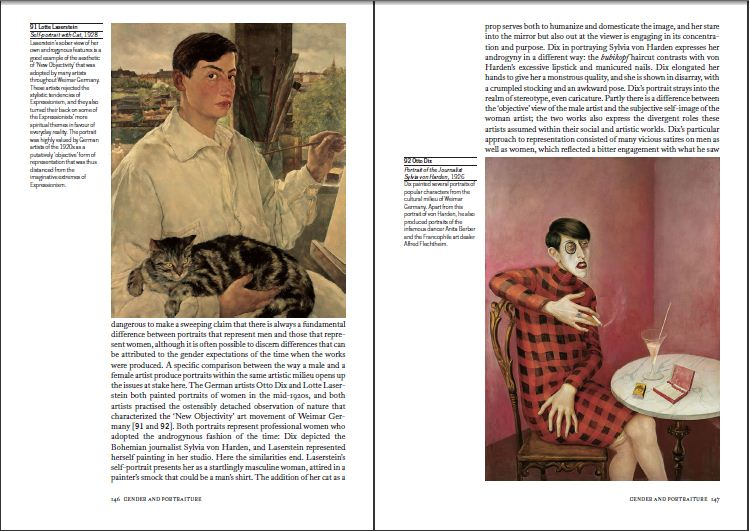
\includegraphics[width=0.7\textwidth]{2-unequal}
  \caption{Unequal width images, they look better if one is up and the other down. Is there a rule? Smaller on top?}
\end{figure}

\begin{figure}[b]
  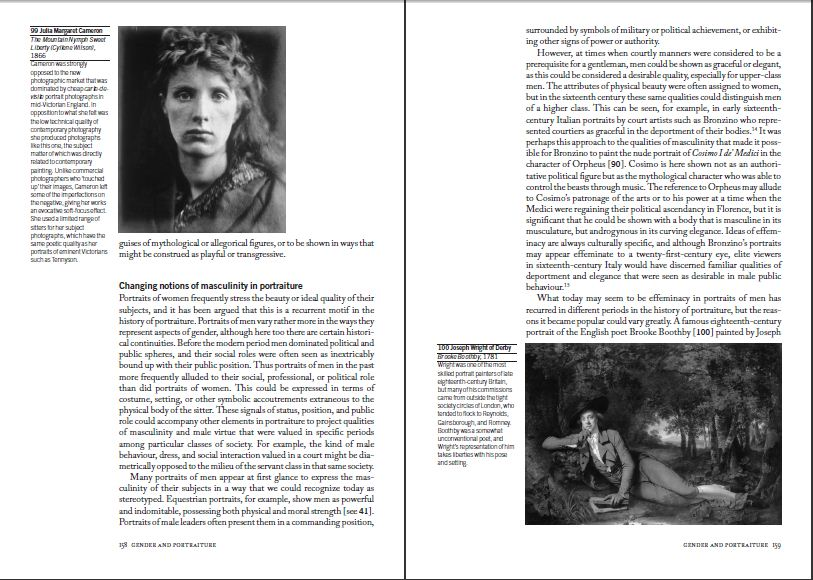
\includegraphics[width=0.7\textwidth]{2-unequal-01}
  \caption{Unequal width images, they look better if one is up and the other down. Is there a rule? Smaller on top?}
\end{figure}

\begin{figure}[b]
  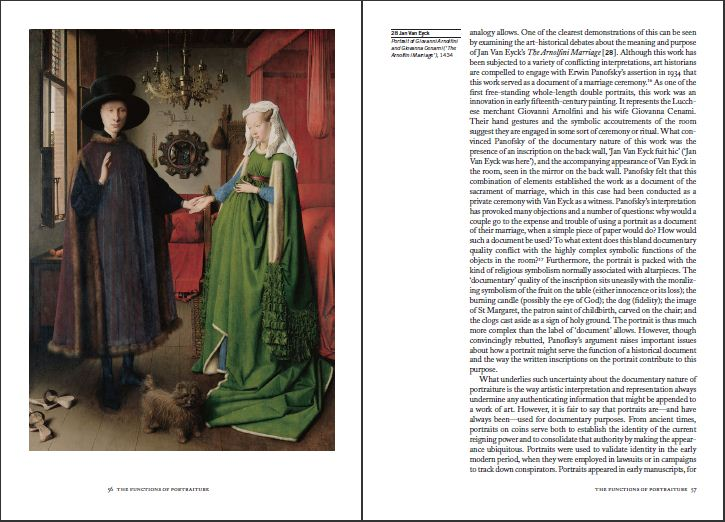
\includegraphics[width=\textwidth]{1-fullpage}
  \caption{Unequal width images, they look better if one is up and the other down. Is there a rule? Smaller on top?}
\end{figure}


\section{Conclusions on single images}
Although the signle images seem to be the easier they are the most difficult to set, as there placement is normally influenced by the image on the following page. Exceptions to the rule abound (the images in black and white are kept smaller) perhaps to defocus them.

\section{Sizing}
In general either fullwidth or textwidth or full page.

\renewcommand{\topfraction}{1}
\begin{figure}[bt]
  \hspace*{-\marginparwidth} 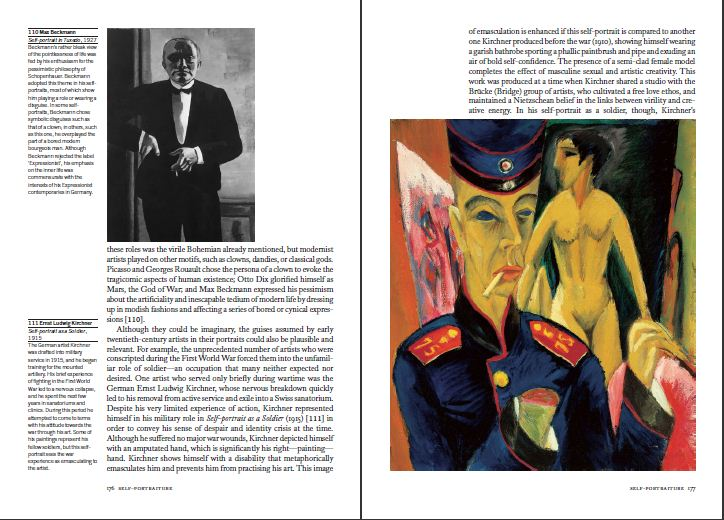
\includegraphics[width=\dimexpr(\textwidth+\marginparwidth)]{2-unequal-02}
  \caption{Unequal width images, they look better if one is up and the other down. Is there a rule? Smaller on top?}
\end{figure}

\clearpage
\lipsum[1-5]
\section{Images before Chapters}
Full page images are difficult to handle in LaTeX. Firstly you need to ensure that they will not trigger a page break (they will if they exceed the textheight). So you need to set  them to pageheight and pagewidth with all page margins etc set to zero. They should start on an even page. Any caption must be placed on the next page in a margin. If not in a margin the next page should have a large section on the bottom footer to insert them. 
\begin{figure}[bt]
  \hspace*{-\marginparwidth} 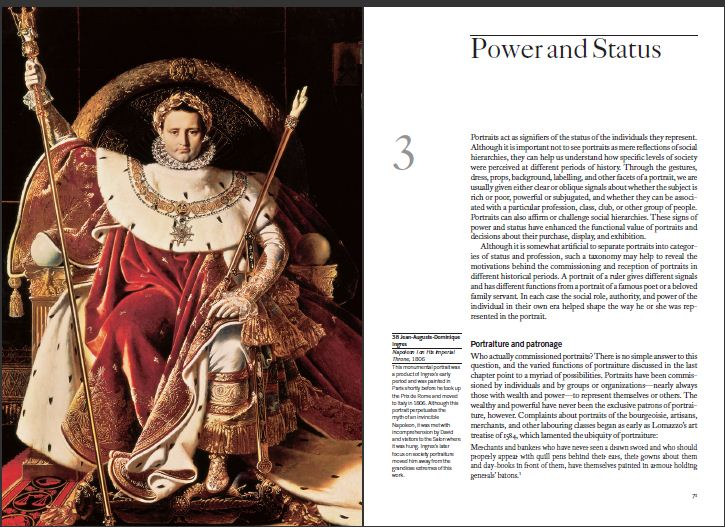
\includegraphics[width=\dimexpr(\textwidth+\marginparwidth)]{1-chapter}
  \caption{Unequal width images, they look better if one is up and the other down. Is there a rule? Smaller on top?}
\end{figure}

\def\fullpageimage{%
    \newgeometry{top=0pt,bottom=0pt,left=0pt, marginparwidth=0pt,marginparsep=0pt,right=0pt}
     \parindent0pt
    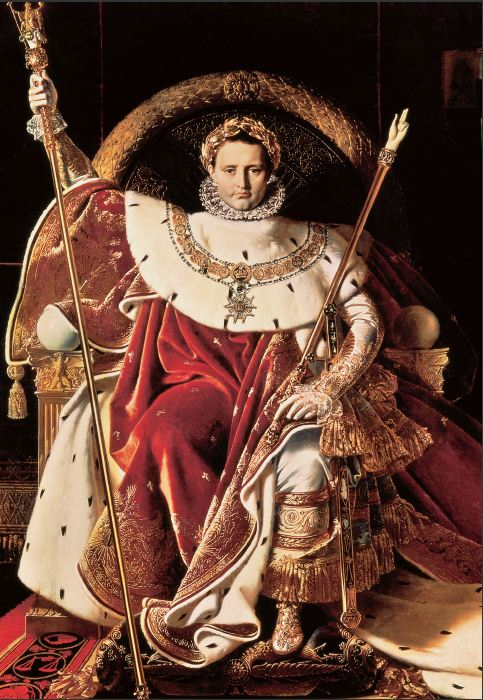
\includegraphics[width=\paperwidth]{napoleon}%
    \restoregeometry%
  }

\fullpageimage
\let\oldplain\ps@plain
\def\restoreplain{\let\ps@plain\oldplain}
\chapter{Napoleon I}
\let\ps@plain\ps@caption
\lipsum[1-7]

\restoreplain

\end{document}